\chapter{Multiresolu��o Sequencial}
\section{Erro Perpendicular}
\section{Erro Tangencial}

\begin{itemize}
  \item {O contorno da elipse $\mathbf{s}_m$ que
  representa o cluster � discretizado num conjunto, $\mathbf{\mathcal C} =
  \{p_1,\ldots,p_8\}$, de $8$ de seus pontos. Espec�ficamente,
  aqueles que definem com o centro da elipse raias que fazem com o eixo maior um �ngulo m�ltiplo de $45^{o}$.  }
\item {Seja  $\mathbf{s}_i$ uma elipse do conjunto $\mathbf{\mathcal T} =
\{\mathbf{s}_1, \ldots,\mathbf{s}_n\}$, que est� sendo condensado e $\mathbf{s}_i^\prime$ um
elipse do conjuto $\mathbf{\mathcal T}^\prime = \{\mathbf{s}_i^\prime,
\ldots,\mathbf{s}_n^\prime\}$\ de elipses projetadas sobre o plano definodo
por $\mathbf{s}_m$. A dist�ncia de cada um dos pontos ($p_{k} \in $ $\mathbf{\mathcal C}$) em que se discretiza 
$\mathbf{s}_m$ a $\mathbf{s}_i^\prime$  $-$ que notaremos por
$dist(p_{k},\mathbf{s}_i^\prime)$ $-$ � obtida de forma aproximada da forma
indicada abaixo. Os elementos referidos no texto a seguir est�o representados na figura X.}
\end{itemize}

\begin{figure}[ht]
\centering
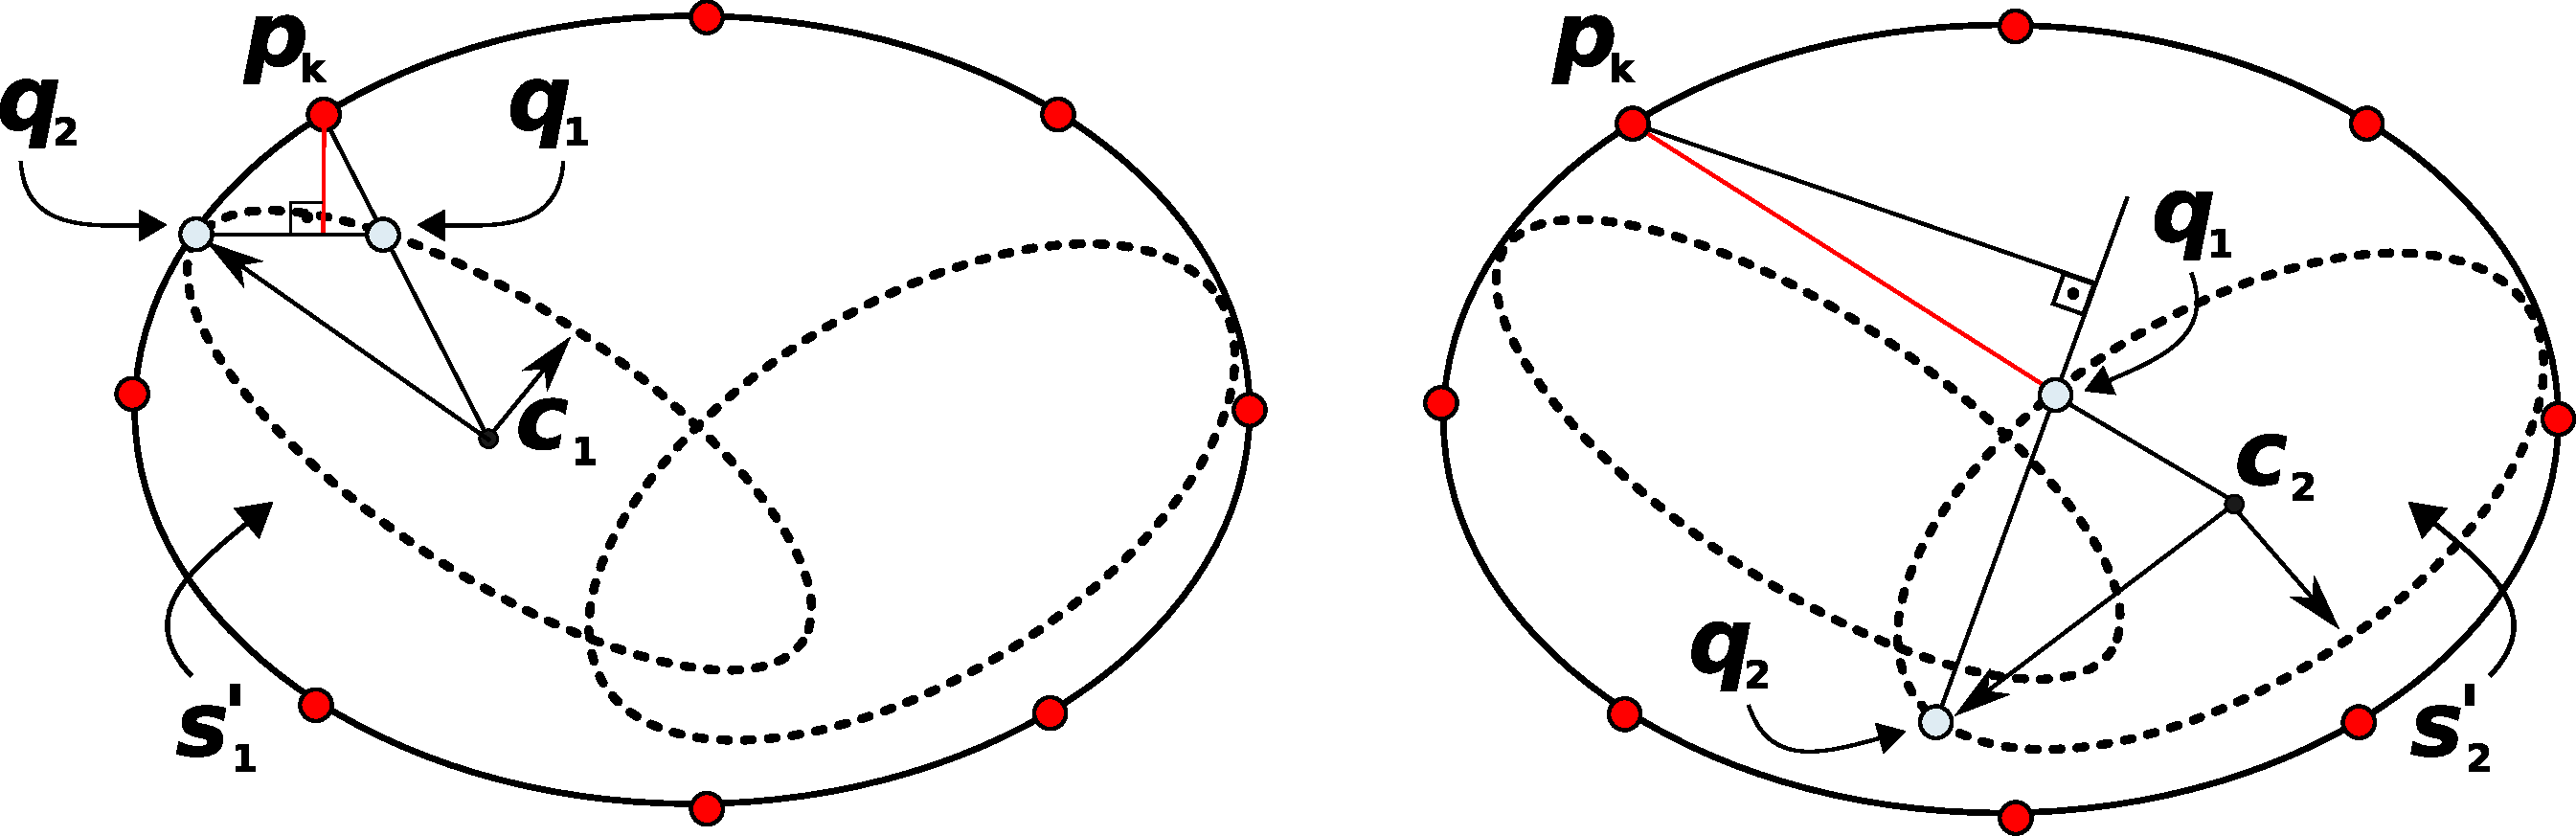
\includegraphics[width=15.0cm]{img/cap05/tangencial} 
\caption{Jun��o dos \textit{splats} de acordo com a m�trica
$\mathbf{\mathit{L}}^2$ (esquerda) e $\mathbf{\mathit{L}}^{2,1}$ (direita) }
\label{fig:merge_splats}
\end{figure}  


\begin{enumerate}
  \item {No caso �bvio em que $p_{k} \in  \mathbf{s}_i^\prime$, teremos
  $dist(p_{k}, \mathbf{s}_i^\prime) = 0 $.}
  \item {Caso contr�rio  considere o segmento de reta delimitado pelo ponto $q_{1}$,  
onde a raia $[ c_{i}, p_{k}]$ corta a elipse  $\mathbf{s}_i^\prime$  e $q_{2}$,  a extremidade do eixo 
maior de $\mathbf{s}_i^\prime$  que est� mais pr�xima de $p_{k}$.}
\item {Computa-se a dist�ncia de  $p_{k}$ a $[q_{1}, q_{2}]$ e usa-se essa dist�ncia como 
aproxima��o de $dist(p_{k}, \mathbf{s}_i^\prime))$. Essa aproxima��o tem erro
percentual limitado por ? e revelou-se suficiente para os prop�sitos de nossa aplica��o.}
\end{enumerate}
 

Utilizando a distancia aproximada definida acima se obtem para cada $p_{k}$
sua dist�ncia ao conjunto de elipses  $\mathbf{\mathcal T}^\prime$ $-$ dado por
$ \min_{ \mathbf{s}_i^\prime \in  \mathbf{\mathcal T}^\prime}
(dist_{p_k \in \mathbf{\mathcal C}}(p_{k}, \mathbf{s}_i^\prime))$. O erro
tangencial ser� finalmente obtido tomando-se a maior dessas dist�ncias. Ele pode, ent�o, ser expresso por:


\begin{eqnarray}
e_t &=& \displaystyle\max  \{ \min_{ \mathbf{s}_i^\prime \in  \mathbf{\mathcal T}^\prime}
(dist_{p_k \in \mathbf{\mathcal C}}(p_{k}, \mathbf{s}_i^\prime)) \}\\\nonumber 
\end{eqnarray}

\section{Resultados}




